\newpage
\section*{Differential Cross Section of Compton Scattering}
The differential cross section of the Compton scattering was derived by Klein and Nishina in 1929 and its expression is:
\begin{equation*}
	\frac{d\sigma}{d\Omega}(\theta)=\frac{r_e ^2}{2}\left(\frac{h \nu_f}{h \nu_i}\right)^2\left(\frac{h \nu_f}{h \nu_i}+\frac{h \nu_i}{h \nu_f}-sen^2(\theta)\right)
\end{equation*}
where $r_e$ is the classical radius of the electron\footnote{$r_e =\dfrac{1}{4\pi \varepsilon_0}\dfrac{e^2}{m_ec^2} =2.82 \times 10^{-15}$ m}.

\medskip

In order to experimentally measure the differential cross section and make a comparison with the theoretical value, the Detector was rotated at 90$^\circ$ and the Scatterer was replaced by an aluminum sample of  diameter $\phi$ 3.4~cm and thickness~h 0.7~cm.  

Initially  a first data acquisition was performed without the aluminum scatterer to store a background spectrum for the two detectors, then the real acquisition was done using the Al sample. For both the session the coincidences between the detectors were used as trigger signals for the digitizer, moreover the total number of events detected by the Tagger was recorded using a CAEN scaler. Fig.~ \ref{Fig:CrossSection_spectra} presents the acquired spectra with and without the aluminum sample. Tagger spectrum does not change with or without the target as expected, instead the Detector spectrum present some differences. The background figure highlight the presence of noise under 200~keV, then a peak around $\sim$250~keV arise with the scattering target, which represents the interested events .

\begin{figure}[h!]
	\centering
	\subfloat[][\text{Detector background spectrum}.]
	{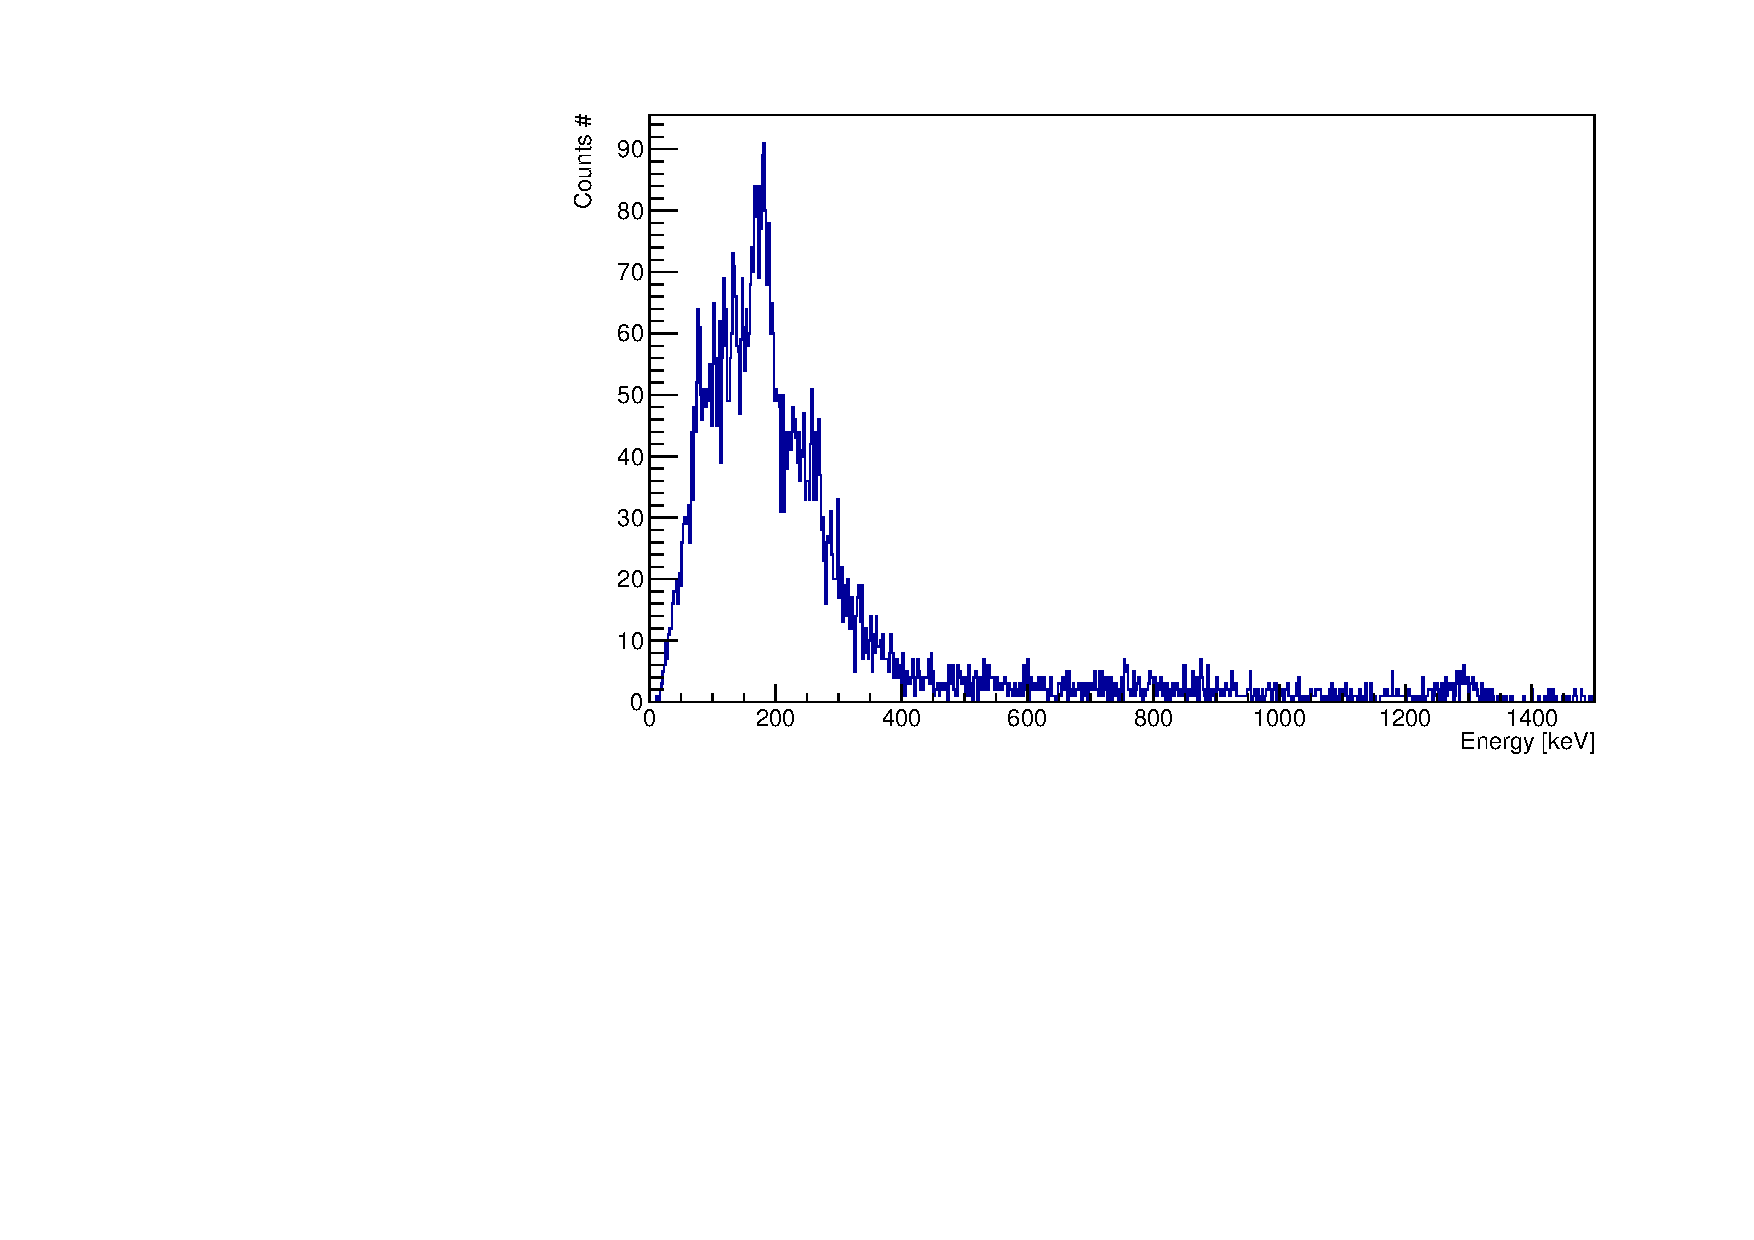
\includegraphics[width=.45\textwidth]{Detector_background}} \quad
	\subfloat[][\text{Detector scattering spectrum}.]
	{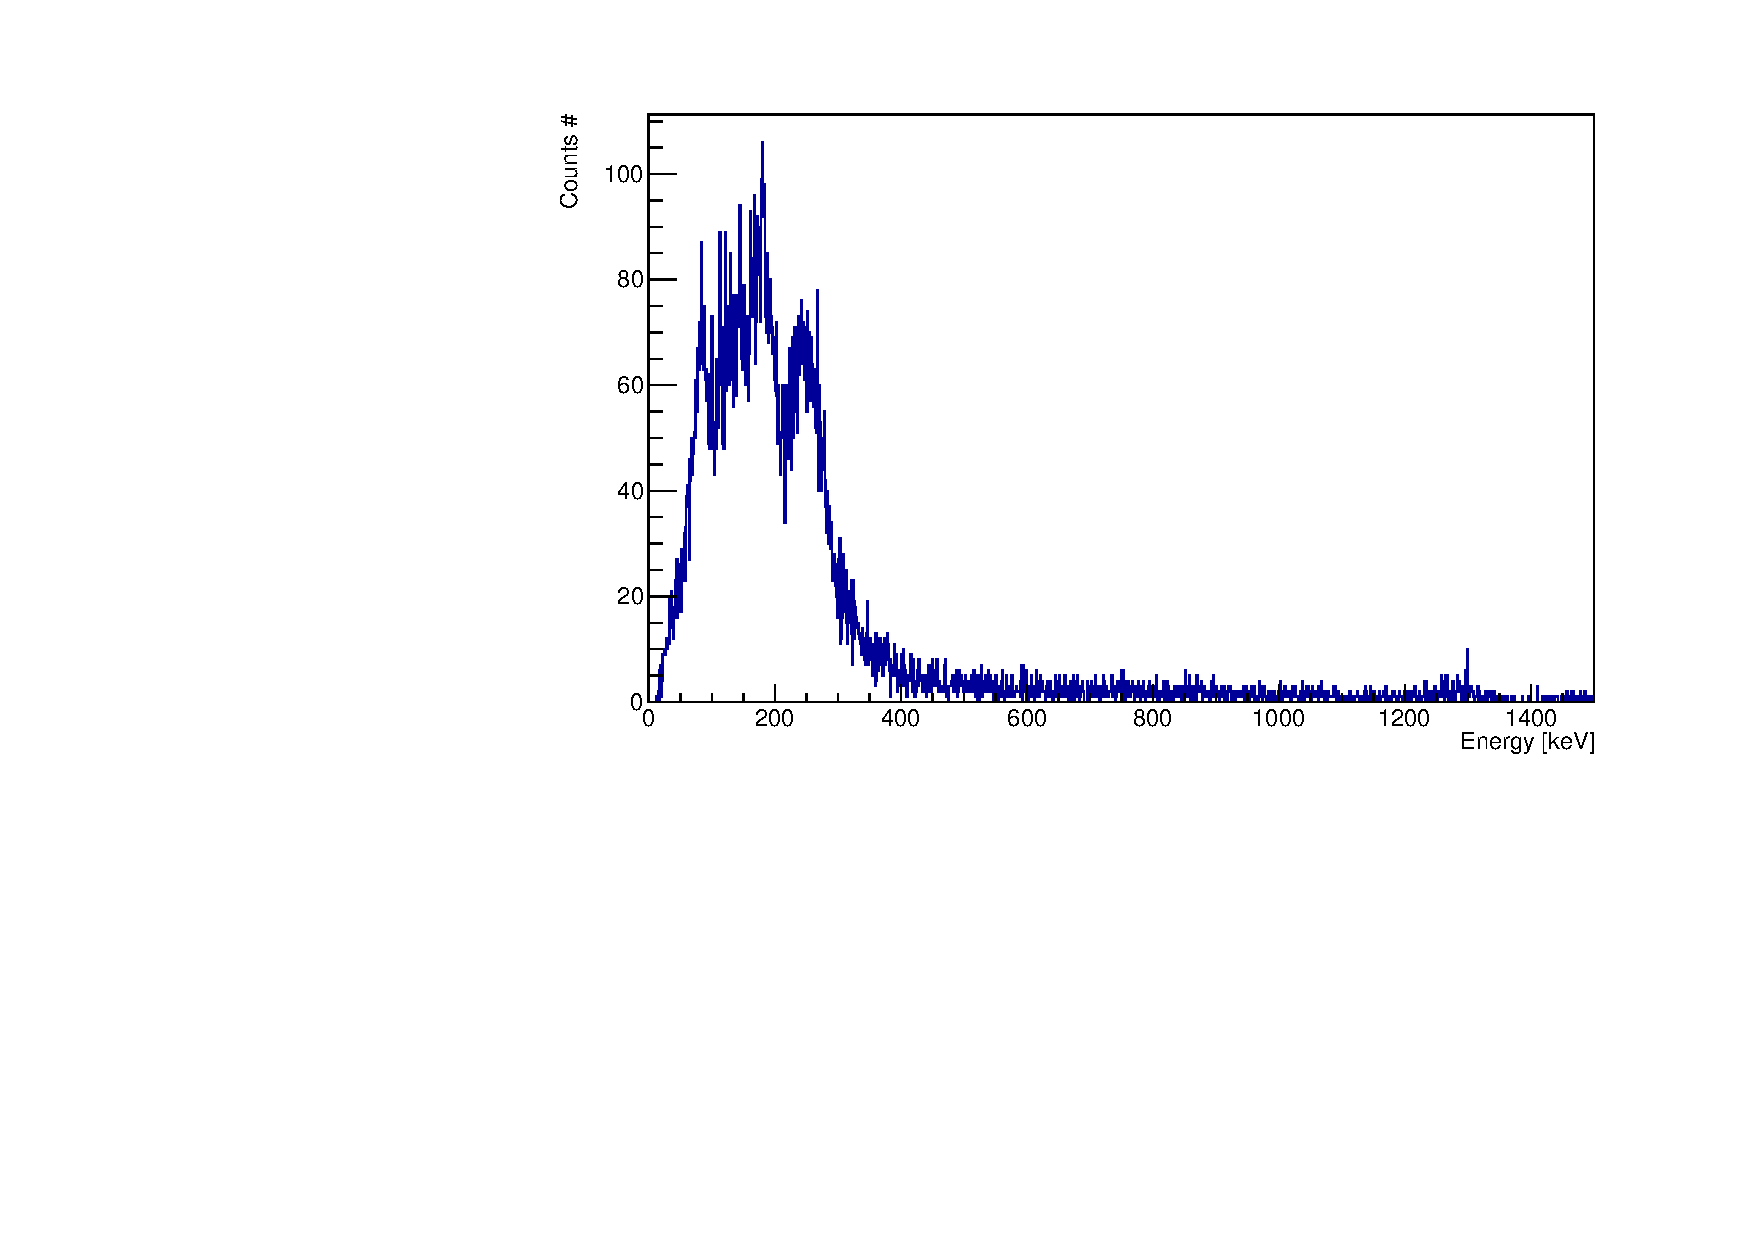
\includegraphics[width=.45\textwidth]{Detector_cross}} \quad
	\subfloat[][\text{Tagger background spectrum }.]
	{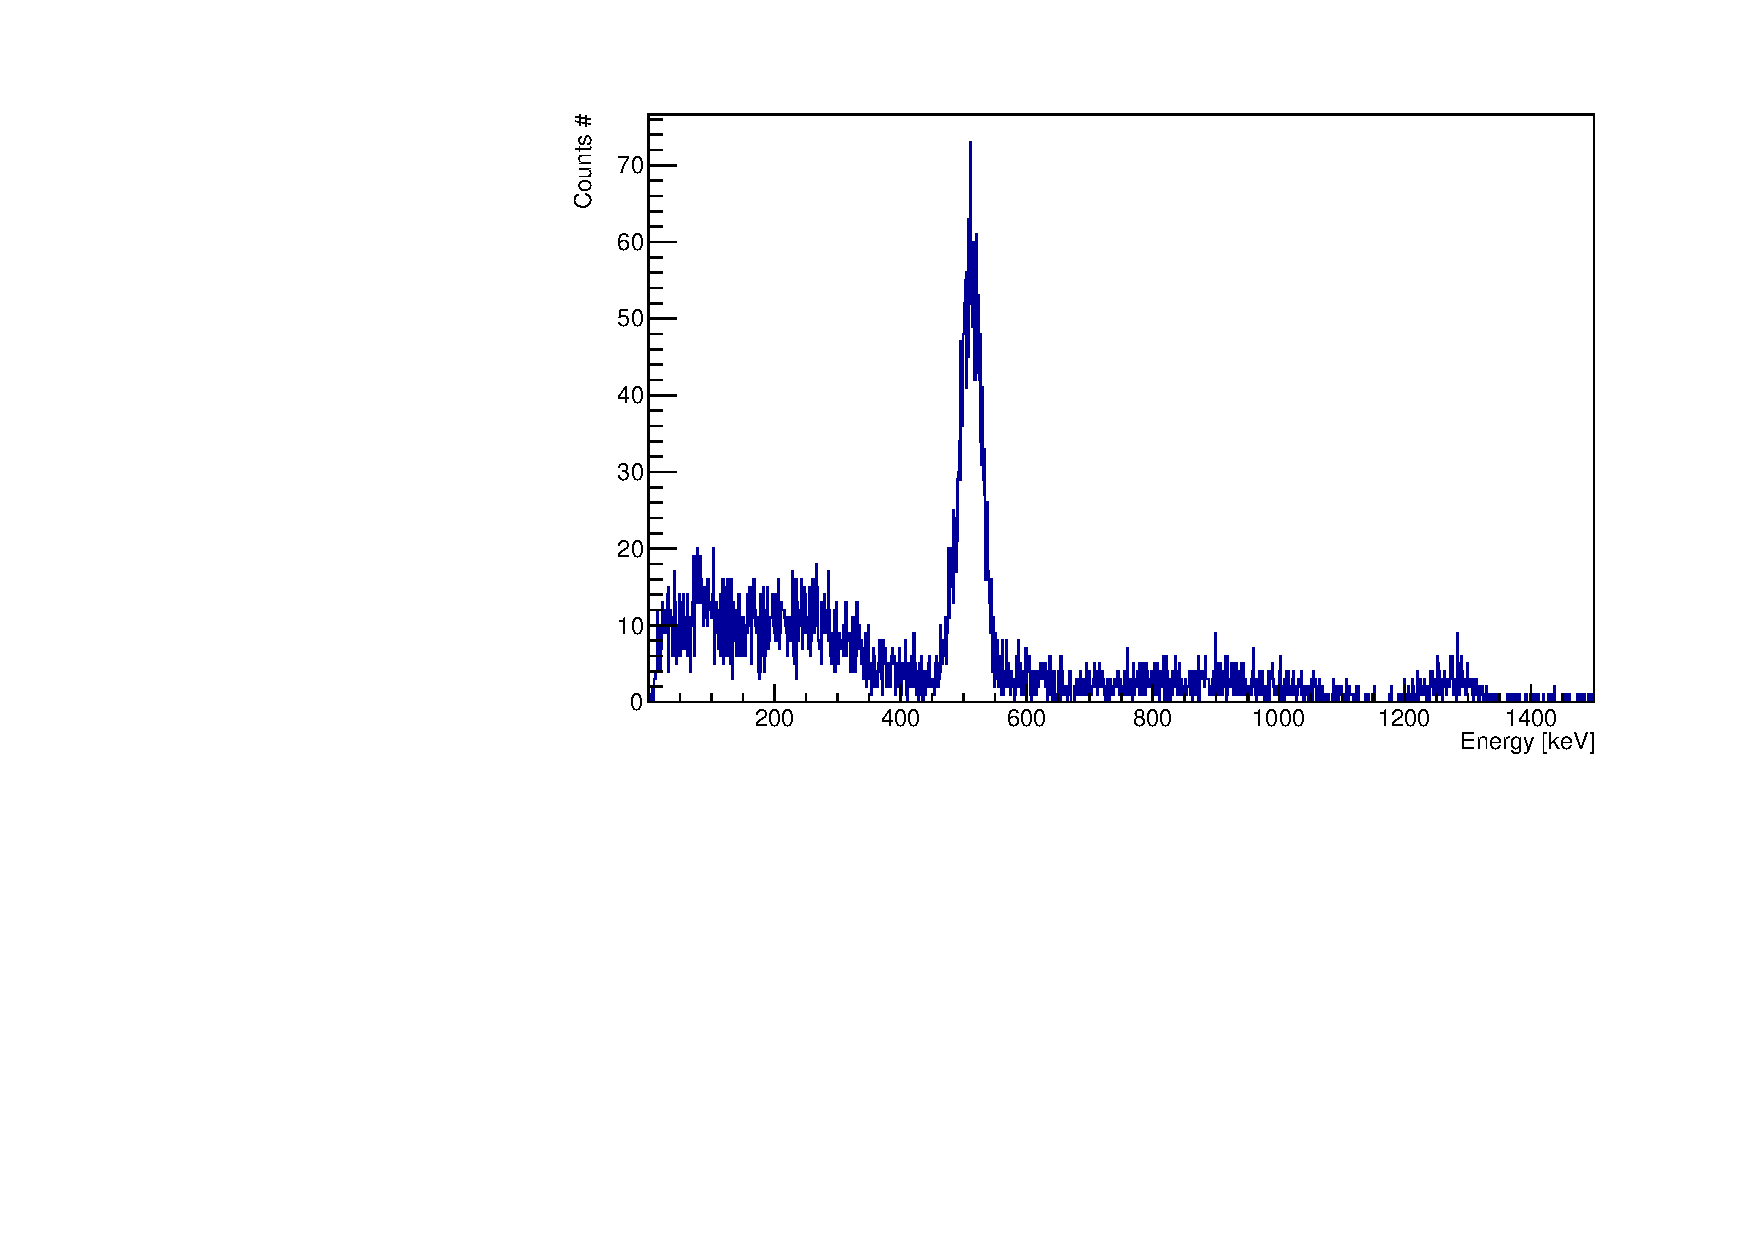
\includegraphics[width=.45\textwidth]{Tagger_background}} \quad
	\subfloat[][\text{Tagger scattering spectrum }.]
	{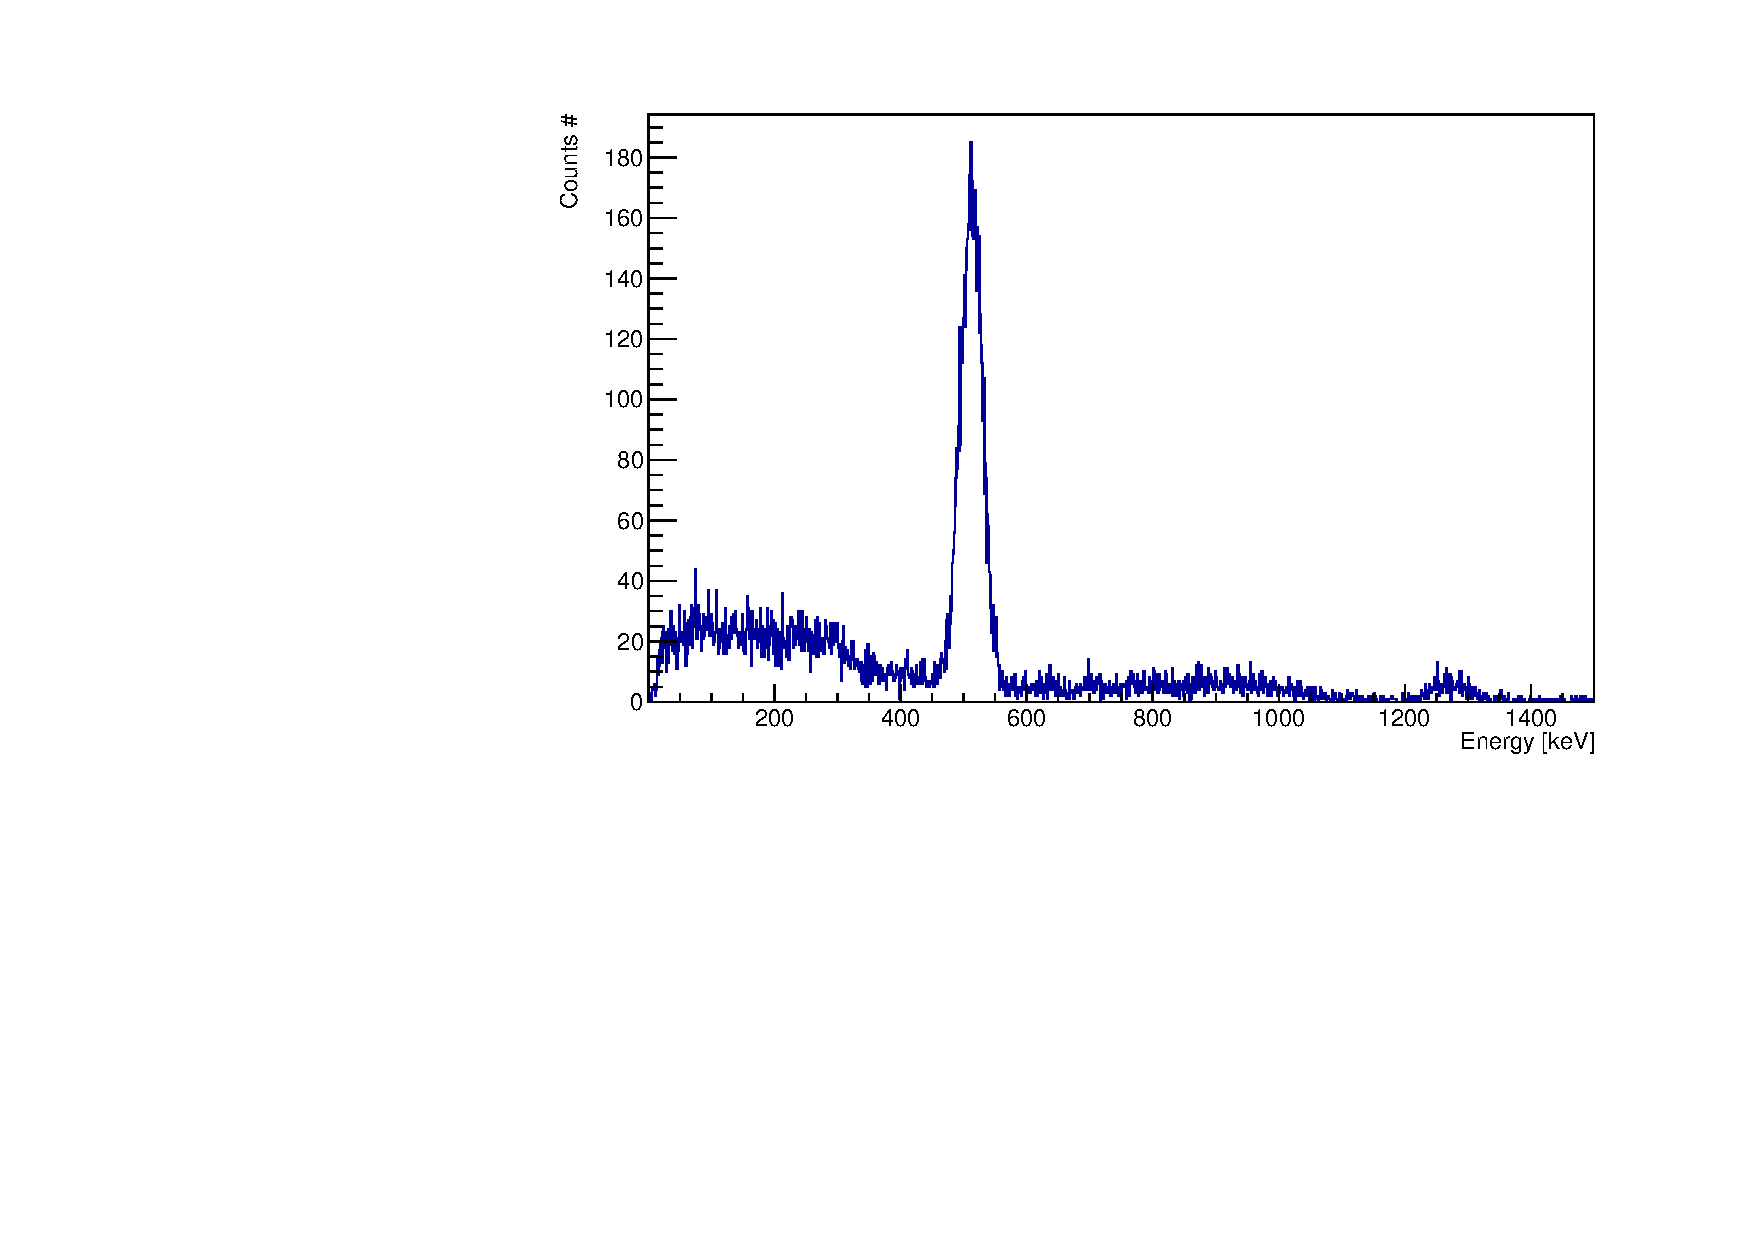
\includegraphics[width=.45\textwidth]{Tagger_cross}}\\
	\caption{Tagger and Detector spectra obtained using an aluminum target as scattering center, the background measurements were performed without the target.}
	\label{Fig:CrossSection_spectra}
\end{figure}
\newpage

The experimental cross section was then calculated as:
\begin{equation*}
	\left[\frac{d\sigma}{d\Omega}(\theta)\right]_{exp}=\frac{\Sigma_\gamma}{\varepsilon\ N\ \Delta\Omega\ I/S}
\end{equation*}
 where $\Sigma_\gamma$ is the number of events in the full energy peak in the spectrum of scattered $\gamma$, $\varepsilon$ is the photopeak efficiency for the energy of scattered  $\gamma$, $N$ is the number of electrons in the sample of Al, $\Delta\Omega$ is the solid angle covered by the Detector, and $I/S$ is the number of $\gamma$ hitting the sample per unit of surface. 
 
 
\subsubsection*{Photopeak efficiency}
Photopeak efficiency $\varepsilon$ was measured positioning Detector and Tagger in contact with the lead collimator, then a data acquisition was performed using as trigger the coincidence between the two detectors.
 $\varepsilon$ was finally calculated as the ratio between number of events in the 511~keV energy peak of the Detector after a background removal and total number of events detected by the tagger and resulted 58\%.
 \subsubsection*{Number of electron in the scattering target}
 Number of electrons $N$ inside the Al sample was computed by the means of this expression 
\[
N=V\times \rho\times N_a\times Z/p
\]
with $\rho$ the Al target density, $N_a$ Avogadro number and $p$  the atomic weight, finding $N=(5.7 \pm 0.3)\cdot10^{24}$ electrons. The following value are used:
\begin{table}[H]
\centering
\begin{tabular}{ll}
\toprule
\toprule
V [cm$^3$] & 6.35 \\
$\rho$ [g/cm$^3$] & 2.6989\\
Z & 26 \\
p & 26.98 \\
$N_a$ & 6.022$\times 10^{23}$ \\
\bottomrule
\bottomrule
\end{tabular}
\end{table}
 
\subsubsection*{Solid Angle }
$\Delta\Omega$ was derived from the geometry of the system, using the expression $\pi r^2/R^2$ with $r$ the radius of Detector face and $R$ the distance between Detector and scattering center. It results $(5.44\pm0.01)\cdot 10^{-2} sr$. 
  
\subsubsection*{Number of $\gamma$ that impinges on the target}
To evaluate $I/S$, the parameter $F(511)$ was computed. $F(511)$ represent the ratio of $\gamma$ inside the full 511~keV peak over the total number of events detected by the Tagger. For this computation the $^{22}$Na Tagger calibrated spectra was used, the Compton background due to the 1275~keV emission was evaluated and subtracted in the region 0 - 600~keV in order to consider only the 511~keV $\gamma$, then the integral of the full energy peak was accounted.
Finally $I/S$ was calculated as the product between the parameter above mentioned and the number of detected events by the Tagger measured with the CAEN scaler, all divided by the surface of the Al target finding 
\[2.2\cdot10^{9} \text{pp/m}^2\]
With all the above mentioned parameters the Cross Section was calculated:
  \begin{equation*}
  	\left[\frac{d\sigma}{d\Omega}(90^{\circ})\right]_{exp}=(3.7\pm0.2) \times 10^{-30}\ \text{m}^{2}
  \end{equation*}
  
  
 
